\documentclass{article}

% The LaTeX-to-CNXML translator makes use of Tralics, a LaTeX-to-XML conversion
% utility.  Tralics has implemented all the packages in the LaTeX base directory,
% and it also supports a good number of supplemental LaTeX packages.  These
% supplemental packages are included in the \usepackage{} statements below.
% Packages not in the LaTeX base directory or \usepackage{} statements in this
% template are not supported by Tralics and, hence, not supported by the
% LaTeX-to-CNXML converter.

% If you have a question as to whether a specific LaTeX command is supported,
% please refer to the "HTML Documentation of all TeX commands" section at
% http://www-sop.inria.fr/apics/tralics/.  Here you will find links to manual pages
% organized alphabetically by the first letter of the command.  These pages indicate
% how Tralics handles conversion of each supported command, which informs how the
% LaTeX-to-CNXML translator behaves.

% To prepare your LaTeX document for import, copy the body of that document from its
% source and paste it into this template between the \begin{document} and \end{document}
% statements.  Do not attempt to use any packages other than the ones contained in this
% template.  You may, however, insert user-defined macros directly in this template
% before the \begin{document} statement.  Following this preparation, check to see if
% your template-compliant document can generate a .dvi (.pdf) using latex (pdflatex).
% If so, then your document is ready for import; if not, you must modify your document
% to generate an output file using only the packages supported by Tralics as described
% above.

%Is this in base?
%\usepackage{epsfig}
%\usepackage{epstopdf}

% Tralics supports the following AMS packages
% (see http://www-sop.inria.fr/apics/tralics/packages.html for details on full/partial
% support of package commands)
\usepackage{amsbsy,amscd,amsfonts,amsgen,amsmath,amsopn,amssymb,amstext,amsthm,amsxtra}

% Tralics supports \includegraphics and \scalebox, but not all other graphicx package
% commands; check the web documentation on supported commands before attempting to use
% other commands in the graphicx package:
\usepackage{graphicx}

% We must specifically invoke the verbatim package as follows to direct Tralics to handle
% the verbatim environment properly:
\usepackage{verbatim}

% Tralics also allows the following packages:
% (see http://www-sop.inria.fr/apics/tralics/packages.html for details on full/partial
% support of package commands)

%\usepackage{alltt}
%\usepackage{array}
%\usepackage{bracket}
%\usepackage{calc}
%\usepackage{delarray}
%\usepackage{eucal}
%\usepackage{eufrak}
%\usepackage{fancyverb}
%\usepackage{fix-cm}
%\usepackage{fixltx2e}
%\usepackage{flafter}
%\usepackage{fontenc}
%\usepackage{fp}
%\usepackage{graphpap}
%\usepackage{html}
%\usepackage{ifthen}
%\usepackage{index}
\usepackage[utf8]{inputenc}
%\usepackage{latexsym}
%\usepackage{lipsum}
%\usepackage{makeidx}
%\usepackage{minimal}
%\usepackage{mml}
%\usepackage{natbib}
%\usepackage{newlfont}
%\usepackage{oldlfont}
%\usepackage{shortvrb}
%\usepackage{showidx}
%\usepackage{soul}
%\usepackage{syntonly}
%\usepackage{textcase}
%\usepackage{textcomp}
%\usepackage{tloop}
%\usepackage{theorem}
%\usepackage{upref}

%-------------------------------------------------------------------
% You can insert user-defined macros (using the supported packages
% only) here...
\DeclareUnicodeCharacter{03B2}{\beta}
%-------------------------------------------------------------------

\title{Guide for Visualizing Booth's Multiplication Algorithm}
\date{\today}

\begin{document}

\section{Getting Started with JHAVÉ}
The easiest way to start the visualization for Booth's multiplication algorithm is by going to \emph{http://jhave.org}.
Under the section titled ``Getting Started'' click the button which says ``Click Here to WebStart Me Now!''.
If a dialogue window appears, select the ``Open'' option, rather than ``Save'', and press OK.
If you have any difficulties getting the JHAVÉ client to run, consult the ``Problems with Java WebStart?'' subsection at \emph{http://jhave.org}.

\begin{figure}[h]
\centering
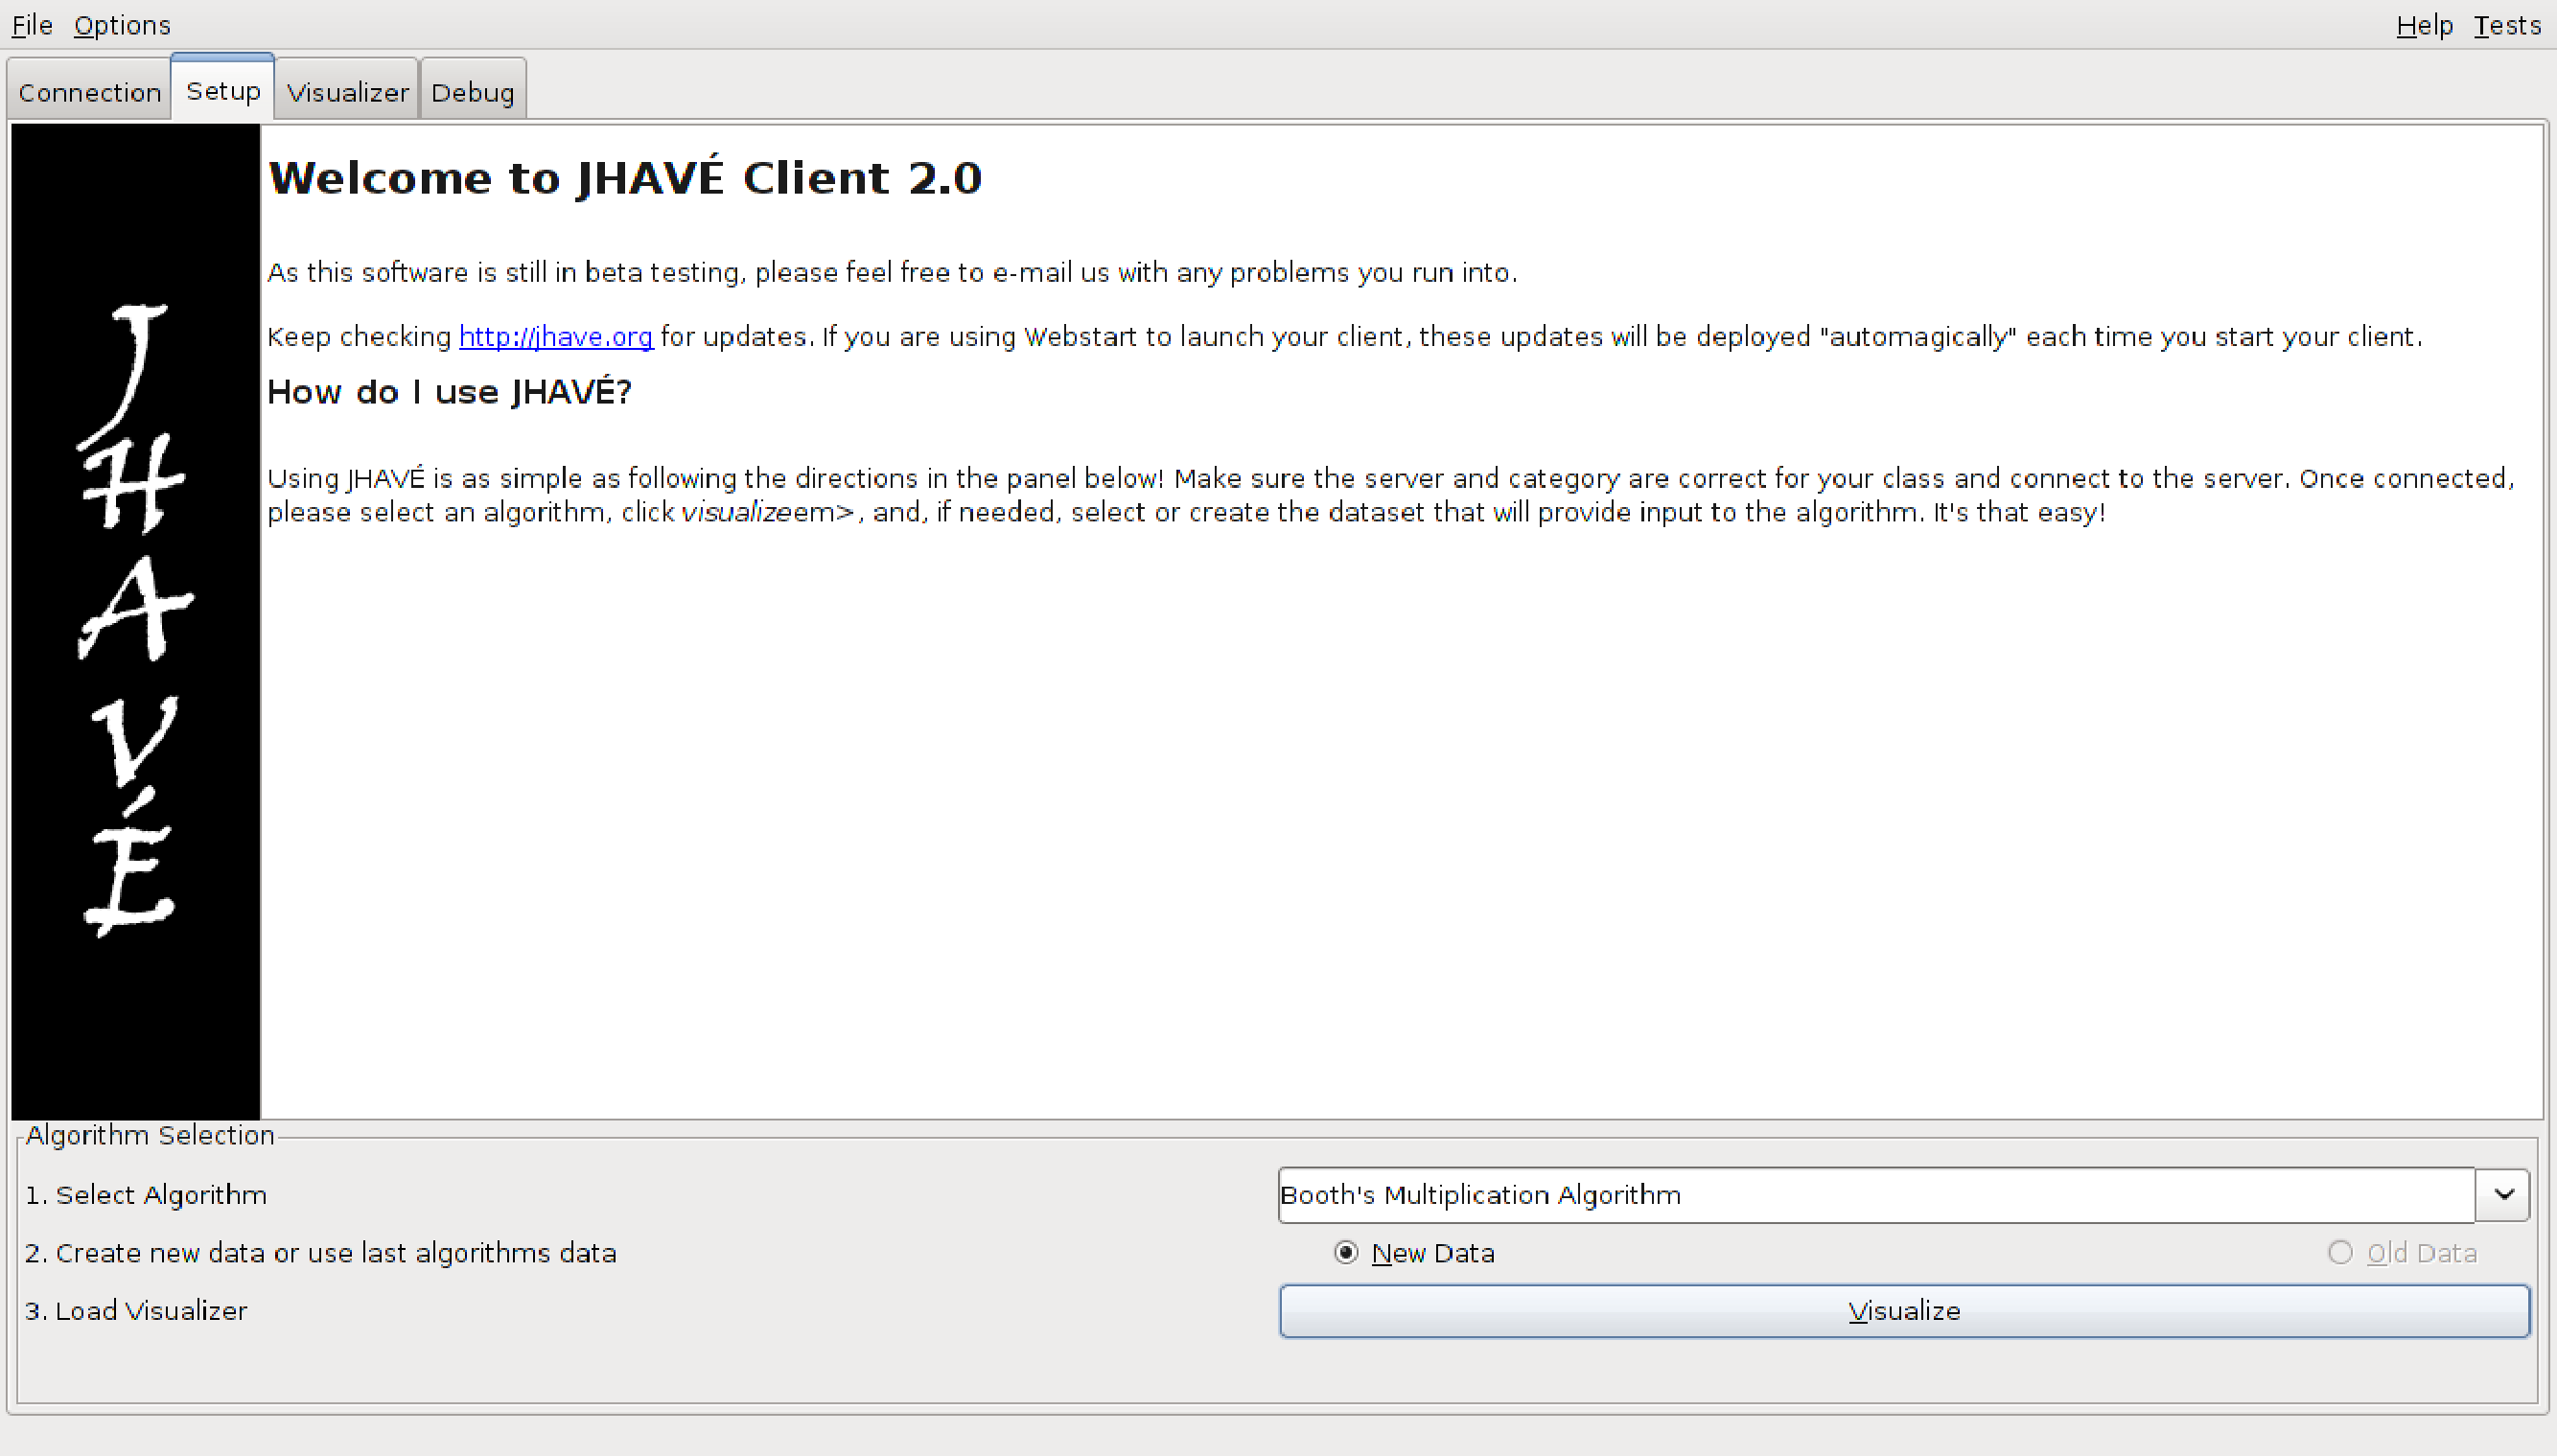
\includegraphics[scale=0.3]{start.pdf}
\caption{The JHAVÉ client}
\end{figure}

\section{The Input Generator}

When the JHAVÉ client is running, select ``Connect''.
On the next screen, select ``Booth's Multiplication Algorithm'' from the drop-down menu of algorithms, and select ``Visualize''.
The algorithm's input generator will appear, with four text fields and a drop-down menu.
The first row of text fields is used to input the multiplicand, and the second row to input the multiplier.
The first column of text fields are for decimal input values, and the second column for binary input values.
Thus, the top-left text field is used to input a decimal value for the multiplicand, and the bottom right text field is used to input a binary value for the multiplier.
Finally, the drop-down menu is used to indicate the number of bits of a register.

\pagebreak

\begin{figure}[h]
\centering
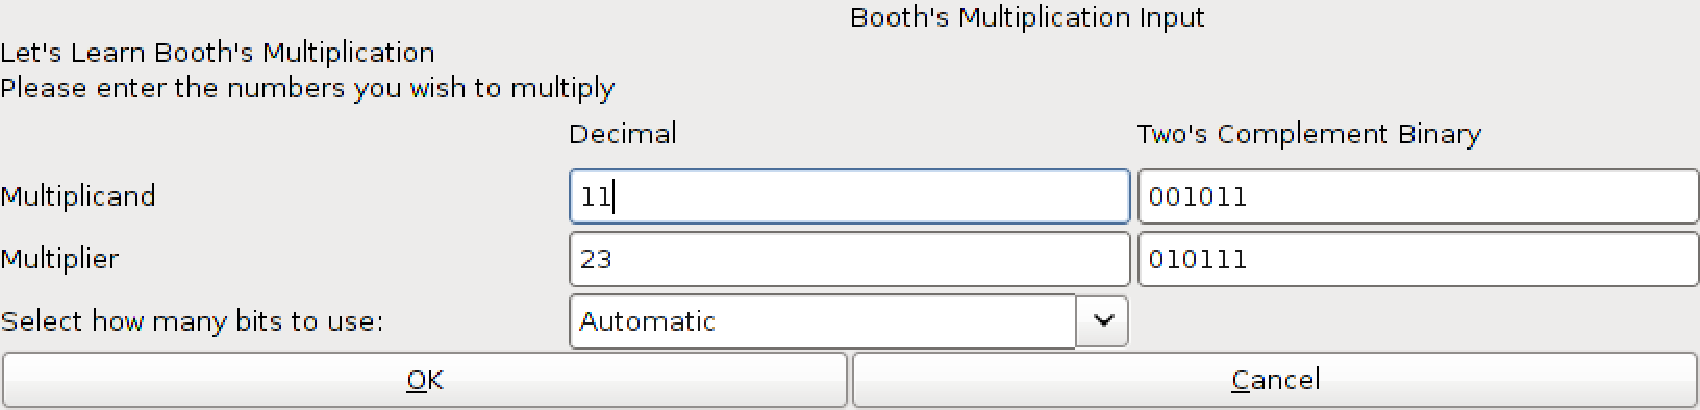
\includegraphics[scale=0.3]{ingen.pdf}
\caption{Booth's Multiplication Algorithm Input Generator}
\end{figure}

Whenever you change one of the values in the four text fields, the input generator will update all text fields according to the input value and register size option selected, or it will signal an error for invalid input.
The ``Automatic'' option will use the least number of bits necessary for the binary representation of both the multiplicand and the multiplier; however, it will never use fewer than 2 bits or greater than 8 bits.
If you select a fixed-register size from the drop-down menu, every value entered in the binary text fields will be resized to the number of bits selected.
If the values entered for the multiplicand or multiplier cannot be represented in the number of bits selected, then an ``Overflow'' error is signalled and the input generator will do its best to correct the mistake, either by using the largest (if you gave a value too large) or smallest (if you gave a value too small) value that can be represented with the selected register size option, or by reverting the the last set of valid values.

\pagebreak
\section{Starting the Visualization}

Once you have selected the desired input values, click ``OK''.
This will take you to the first snapshot of the visualization.
You should see figures depicting decimal and binary multiplication on the top left and top right, respectively.
On the right side of the visualization is an area marked ``Math/ALU''.
Whenever binary addition or subtraction occurs, a diagram appears in this area to show you how the result is derived.
To the right of this is a pane with two tabs.
One tab, titled ``Pseudo Code'' displays pseudo code for the executing algorithm.
For every snapshot, a line in the pseudo code is highlighted indicating what has just happened in the visualization.
Finally, the text in the top center of the screen also provides information about the current step of the visualization.

\begin{figure}[h]
\centering
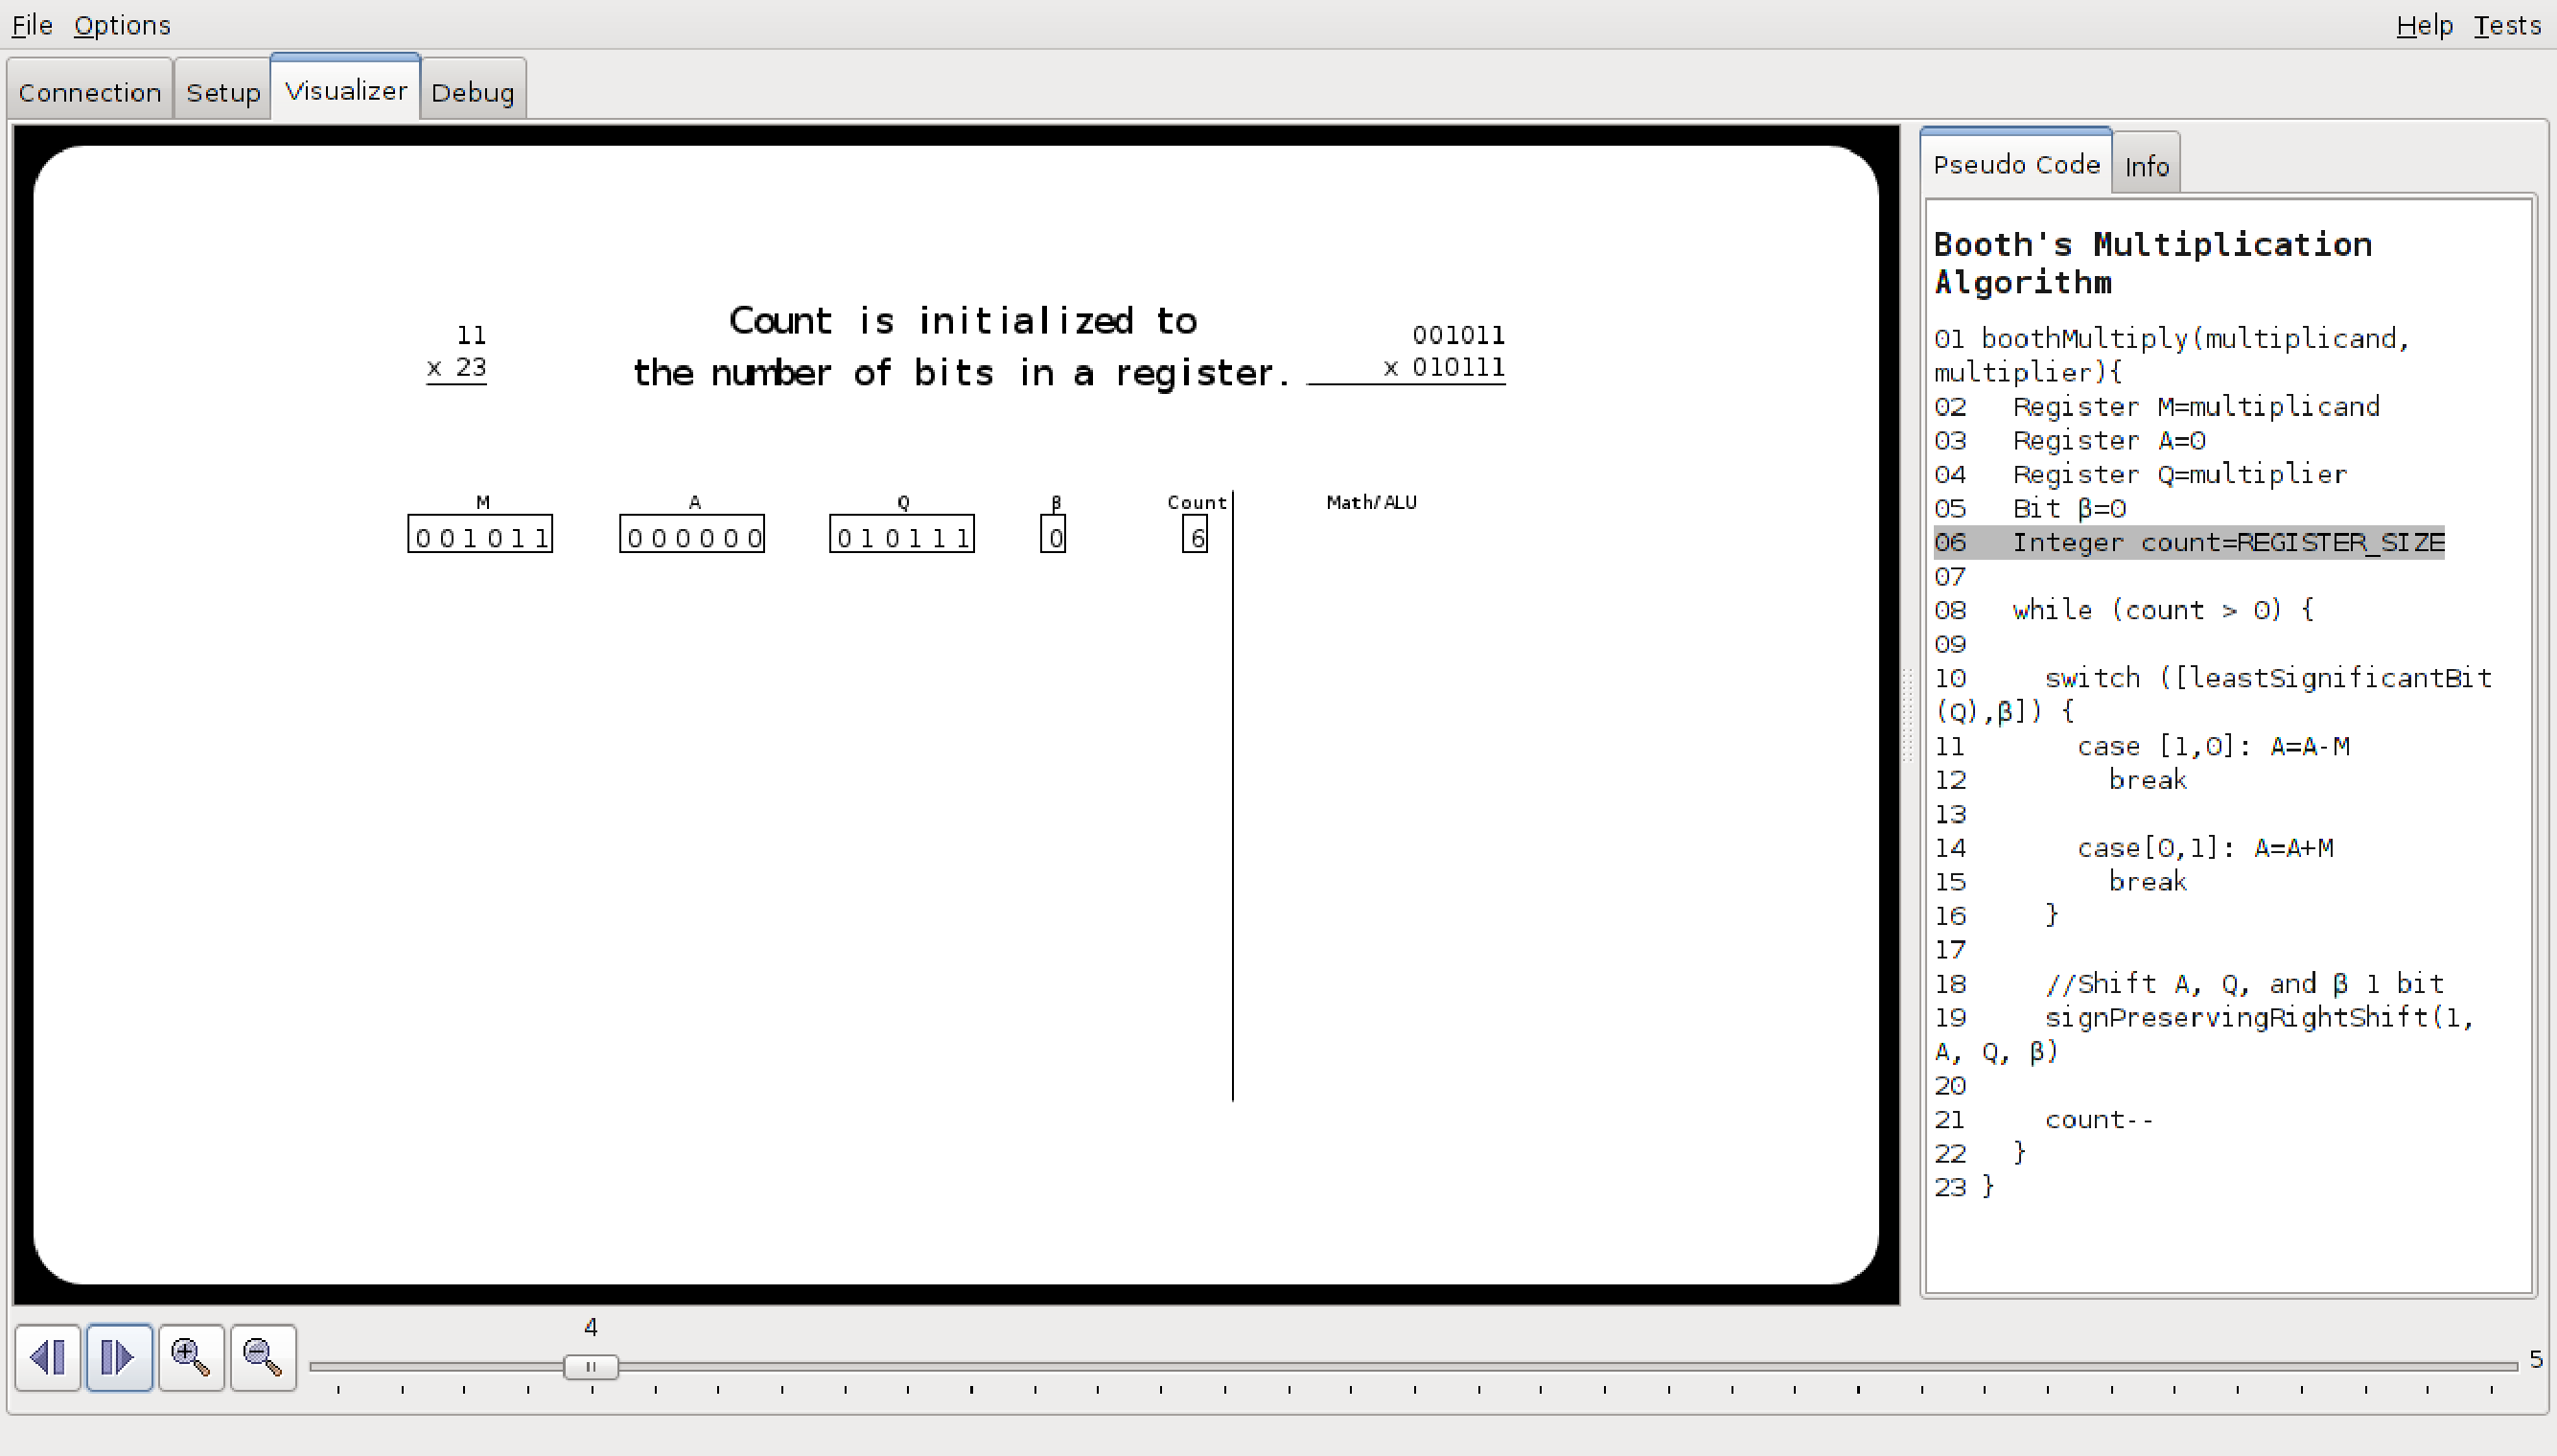
\includegraphics[scale=0.3]{initreg.pdf}
\caption{The Initialization of M, A, Q, \beta, and Count}%it seems fine to use Beta rather than β
\end{figure}

To navigate through the visualization, click the arrow buttons on the bottom left of the screen.
The first few slides are dedicated to setting up the initial values the algorithm will use.
After this, the visualization goes into the loop of the algorithm.

\pagebreak
\begin{figure}[h]
\centering
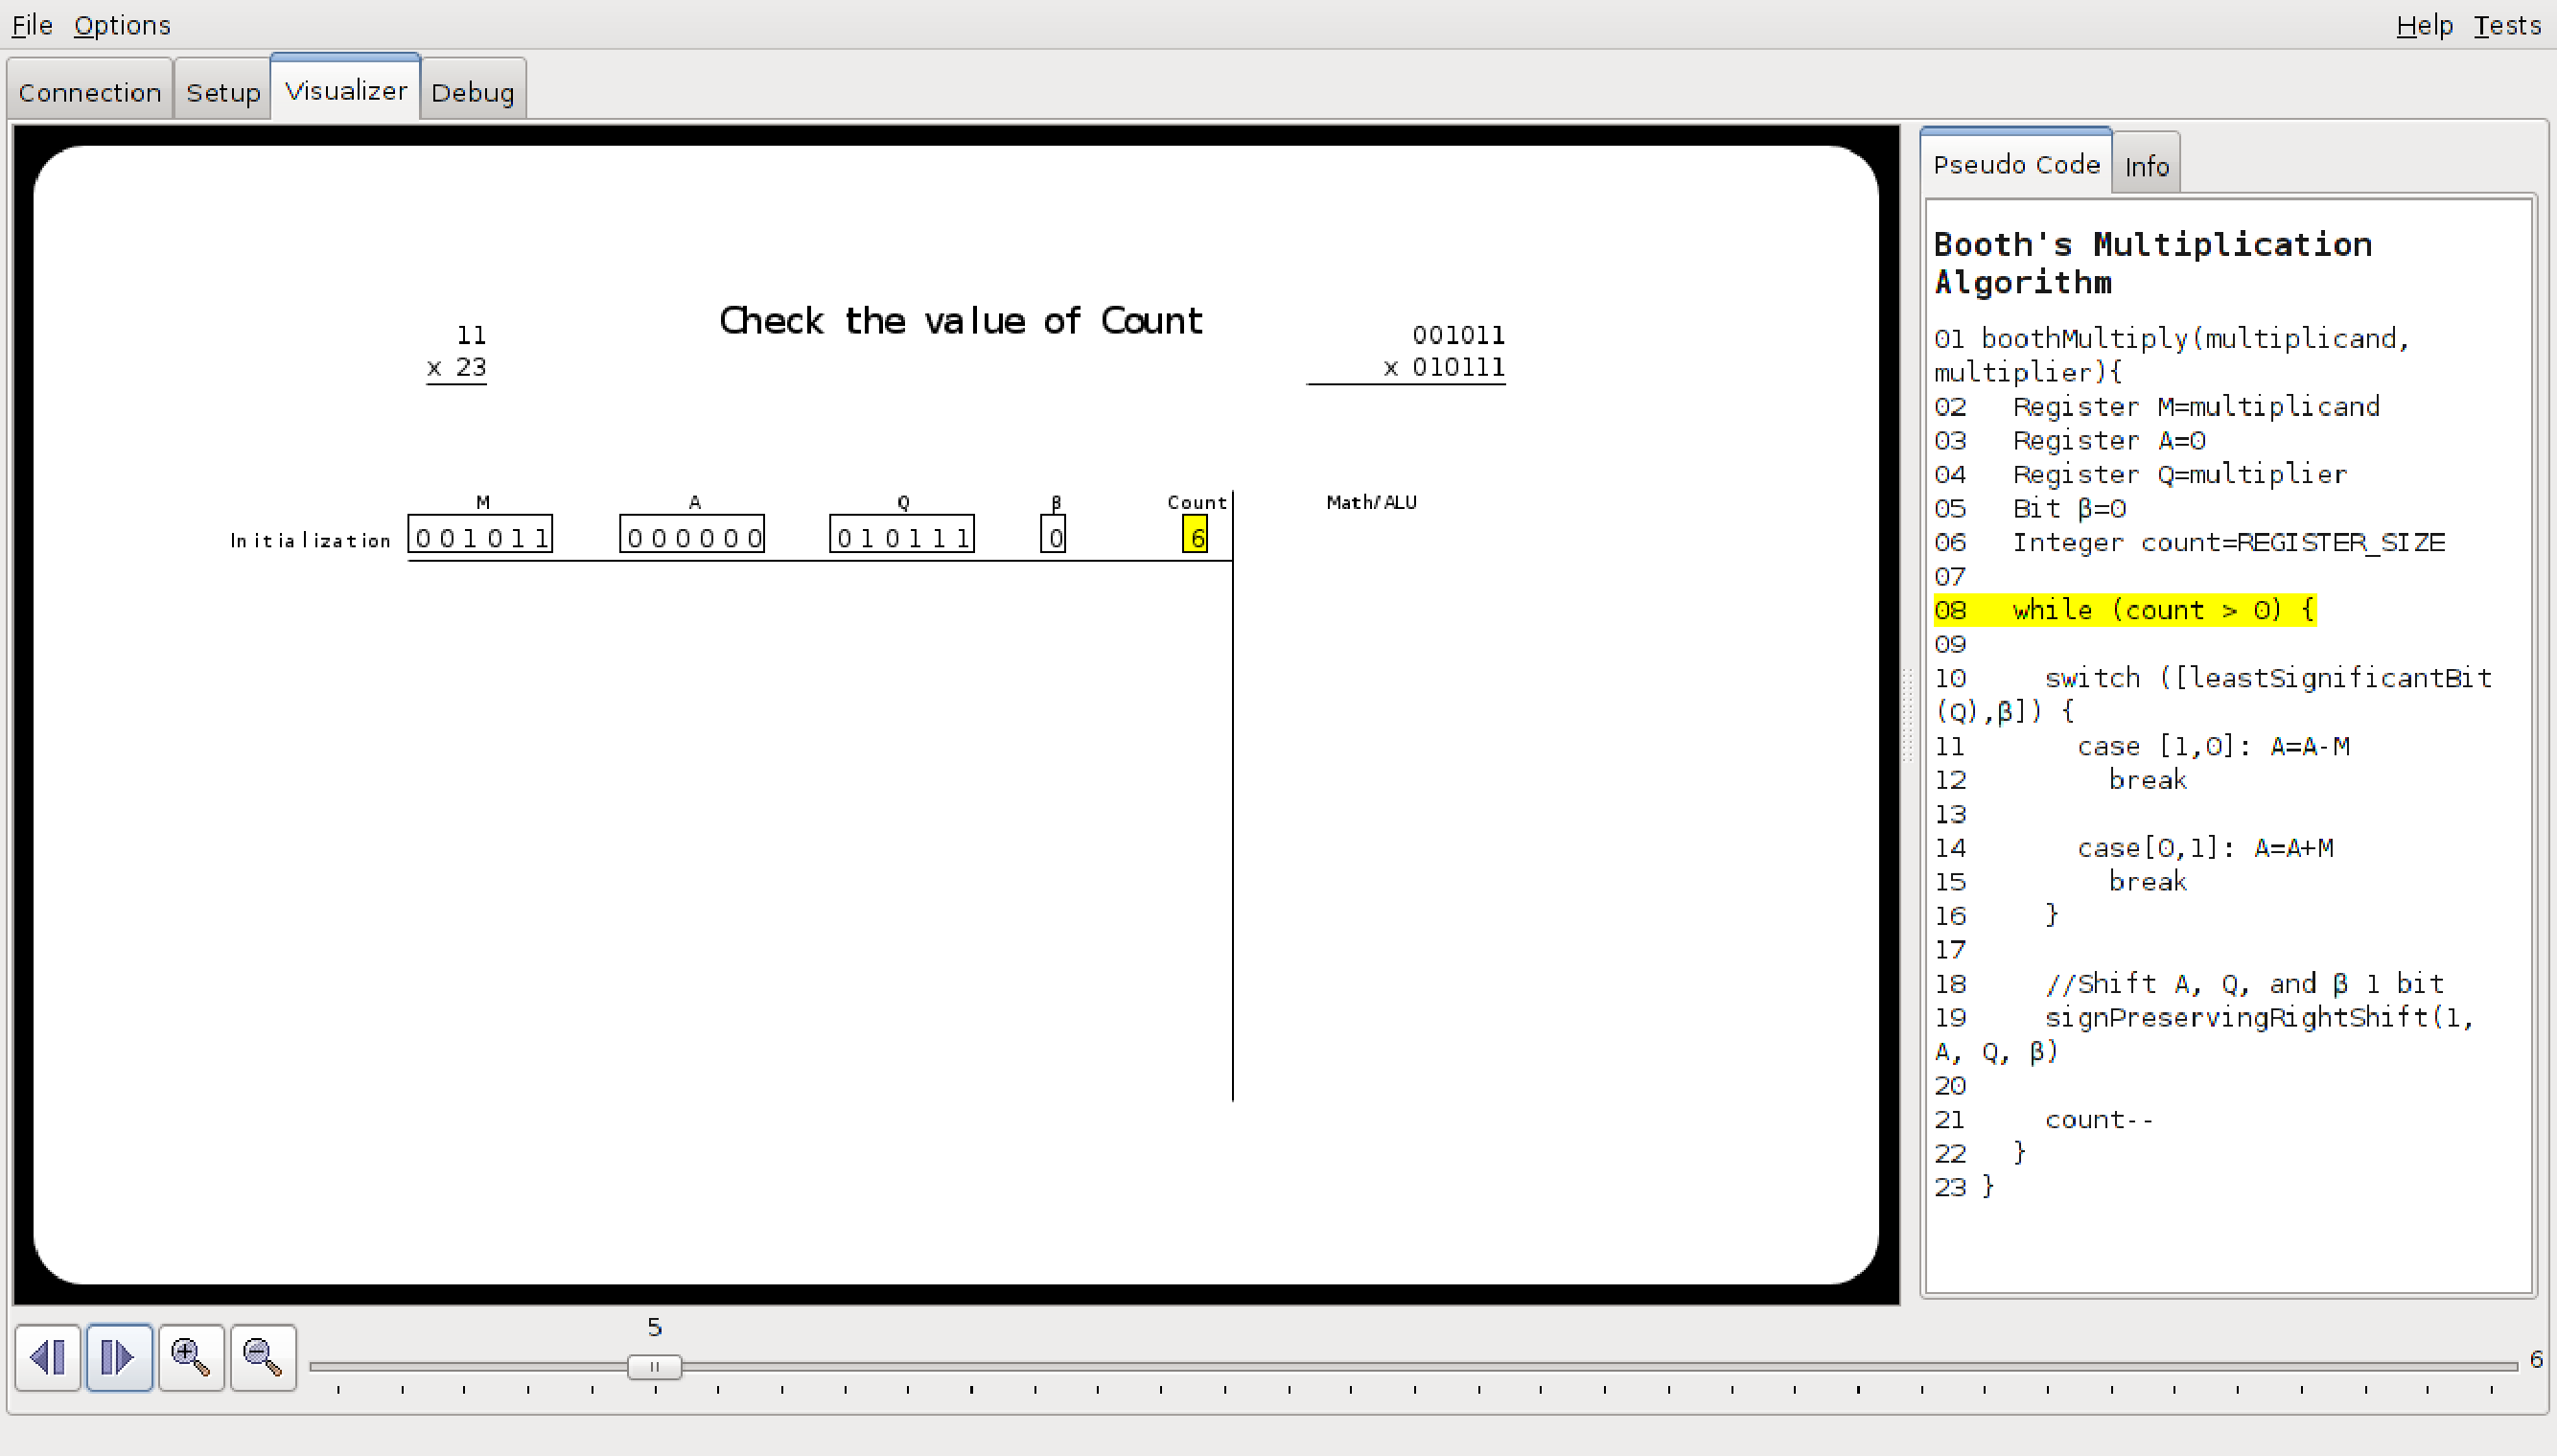
\includegraphics[scale=0.3]{looptop.pdf}
\caption{Beginning of the loop}
\end{figure}

As the visualization progresses, the state history of the algorithm is preserved on screen, along with appropriate annotations to the left of the registers.
The current values for the algorithm are drawn in black text and in black boxes, and values for past states of the algorithm are drawn in grey text in grey boxes.
This is done to allow you to refer to previous states for reference.
Depending on your window size, you may not be able to see the annotations.
If you cannot see these annotations, or if you wish to adjust your view of the visualization in general, you can resize your window if possible, zoom in and out with the magnifying glass buttons on the bottom left, or click and drag the visualization to move it as you like.

\pagebreak
\section{An Example Iteration of the Loop}
Each iteraction of the loop will be one of three cases.
%At the top of the loop, a switch statement is used to determine the case.

\begin{figure}[h]
\centering
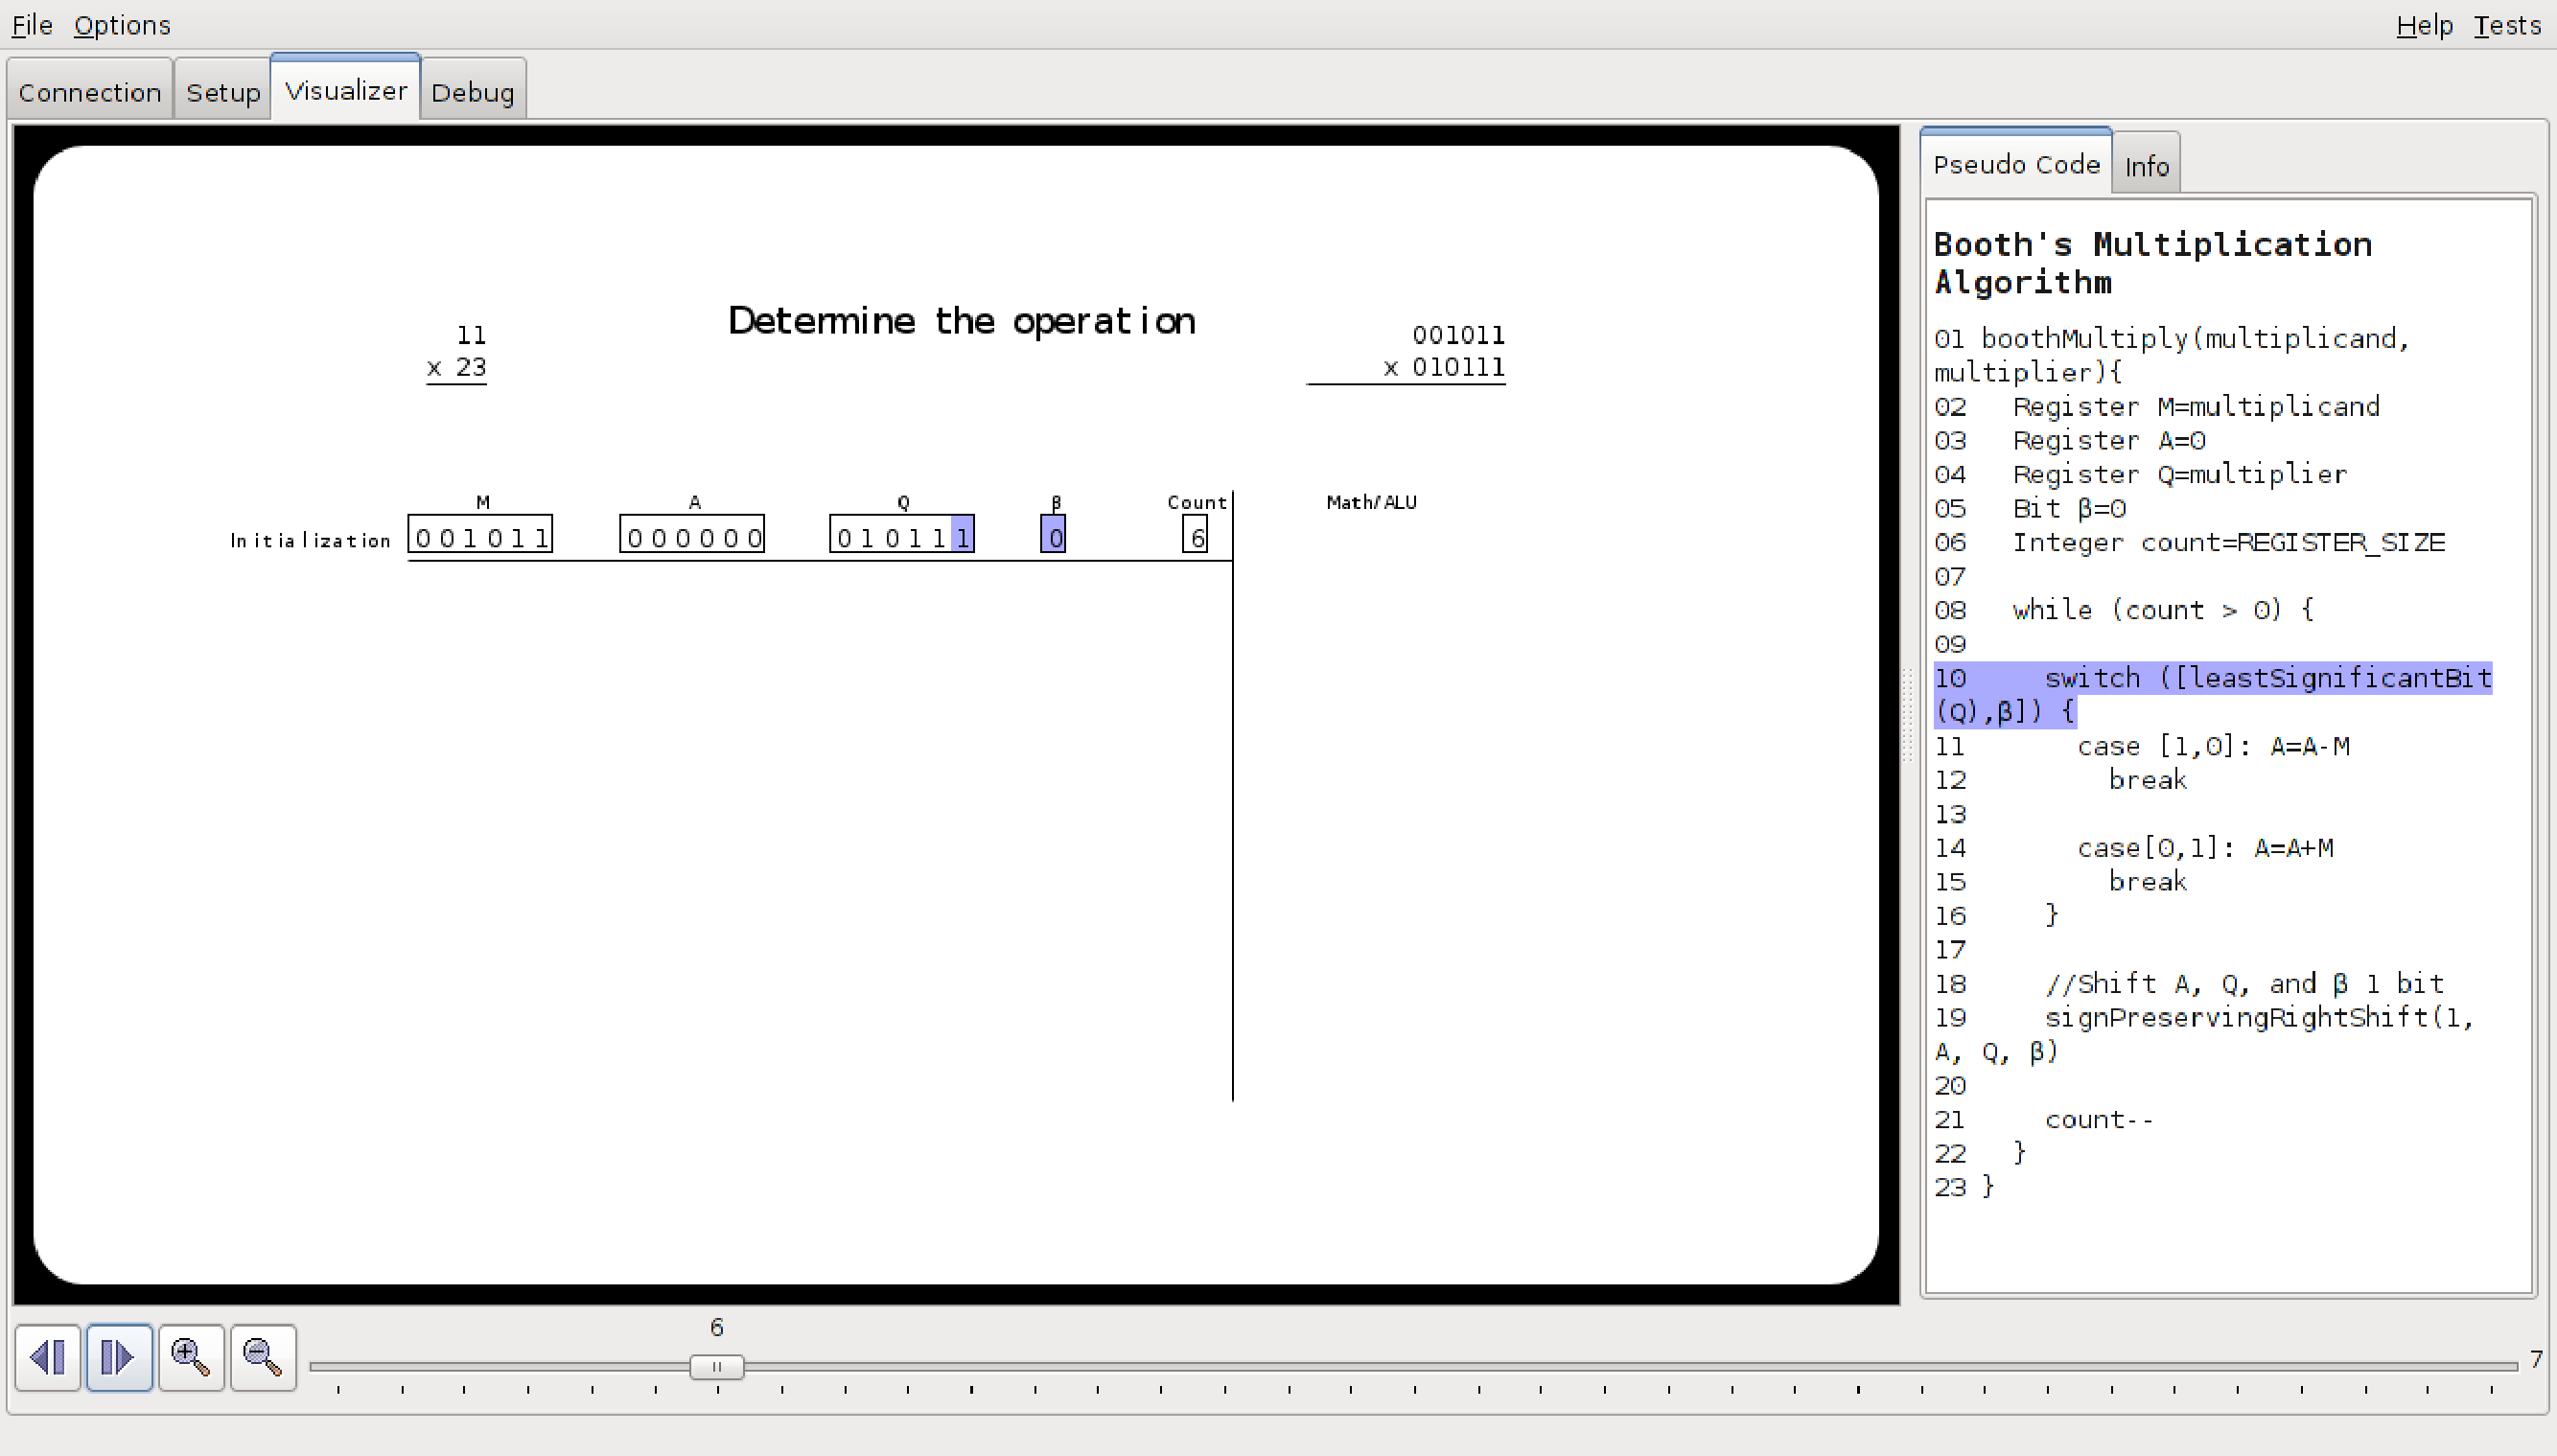
\includegraphics[scale=0.3]{cases.pdf}
\caption{Check the case}
\end{figure}

The bits being compared are highlighted in blue; the corresponding line of pseudo-code is highlighted in blue as well.

\pagebreak
Then the operations for that case are executed:

\begin{figure}[h]
\centering
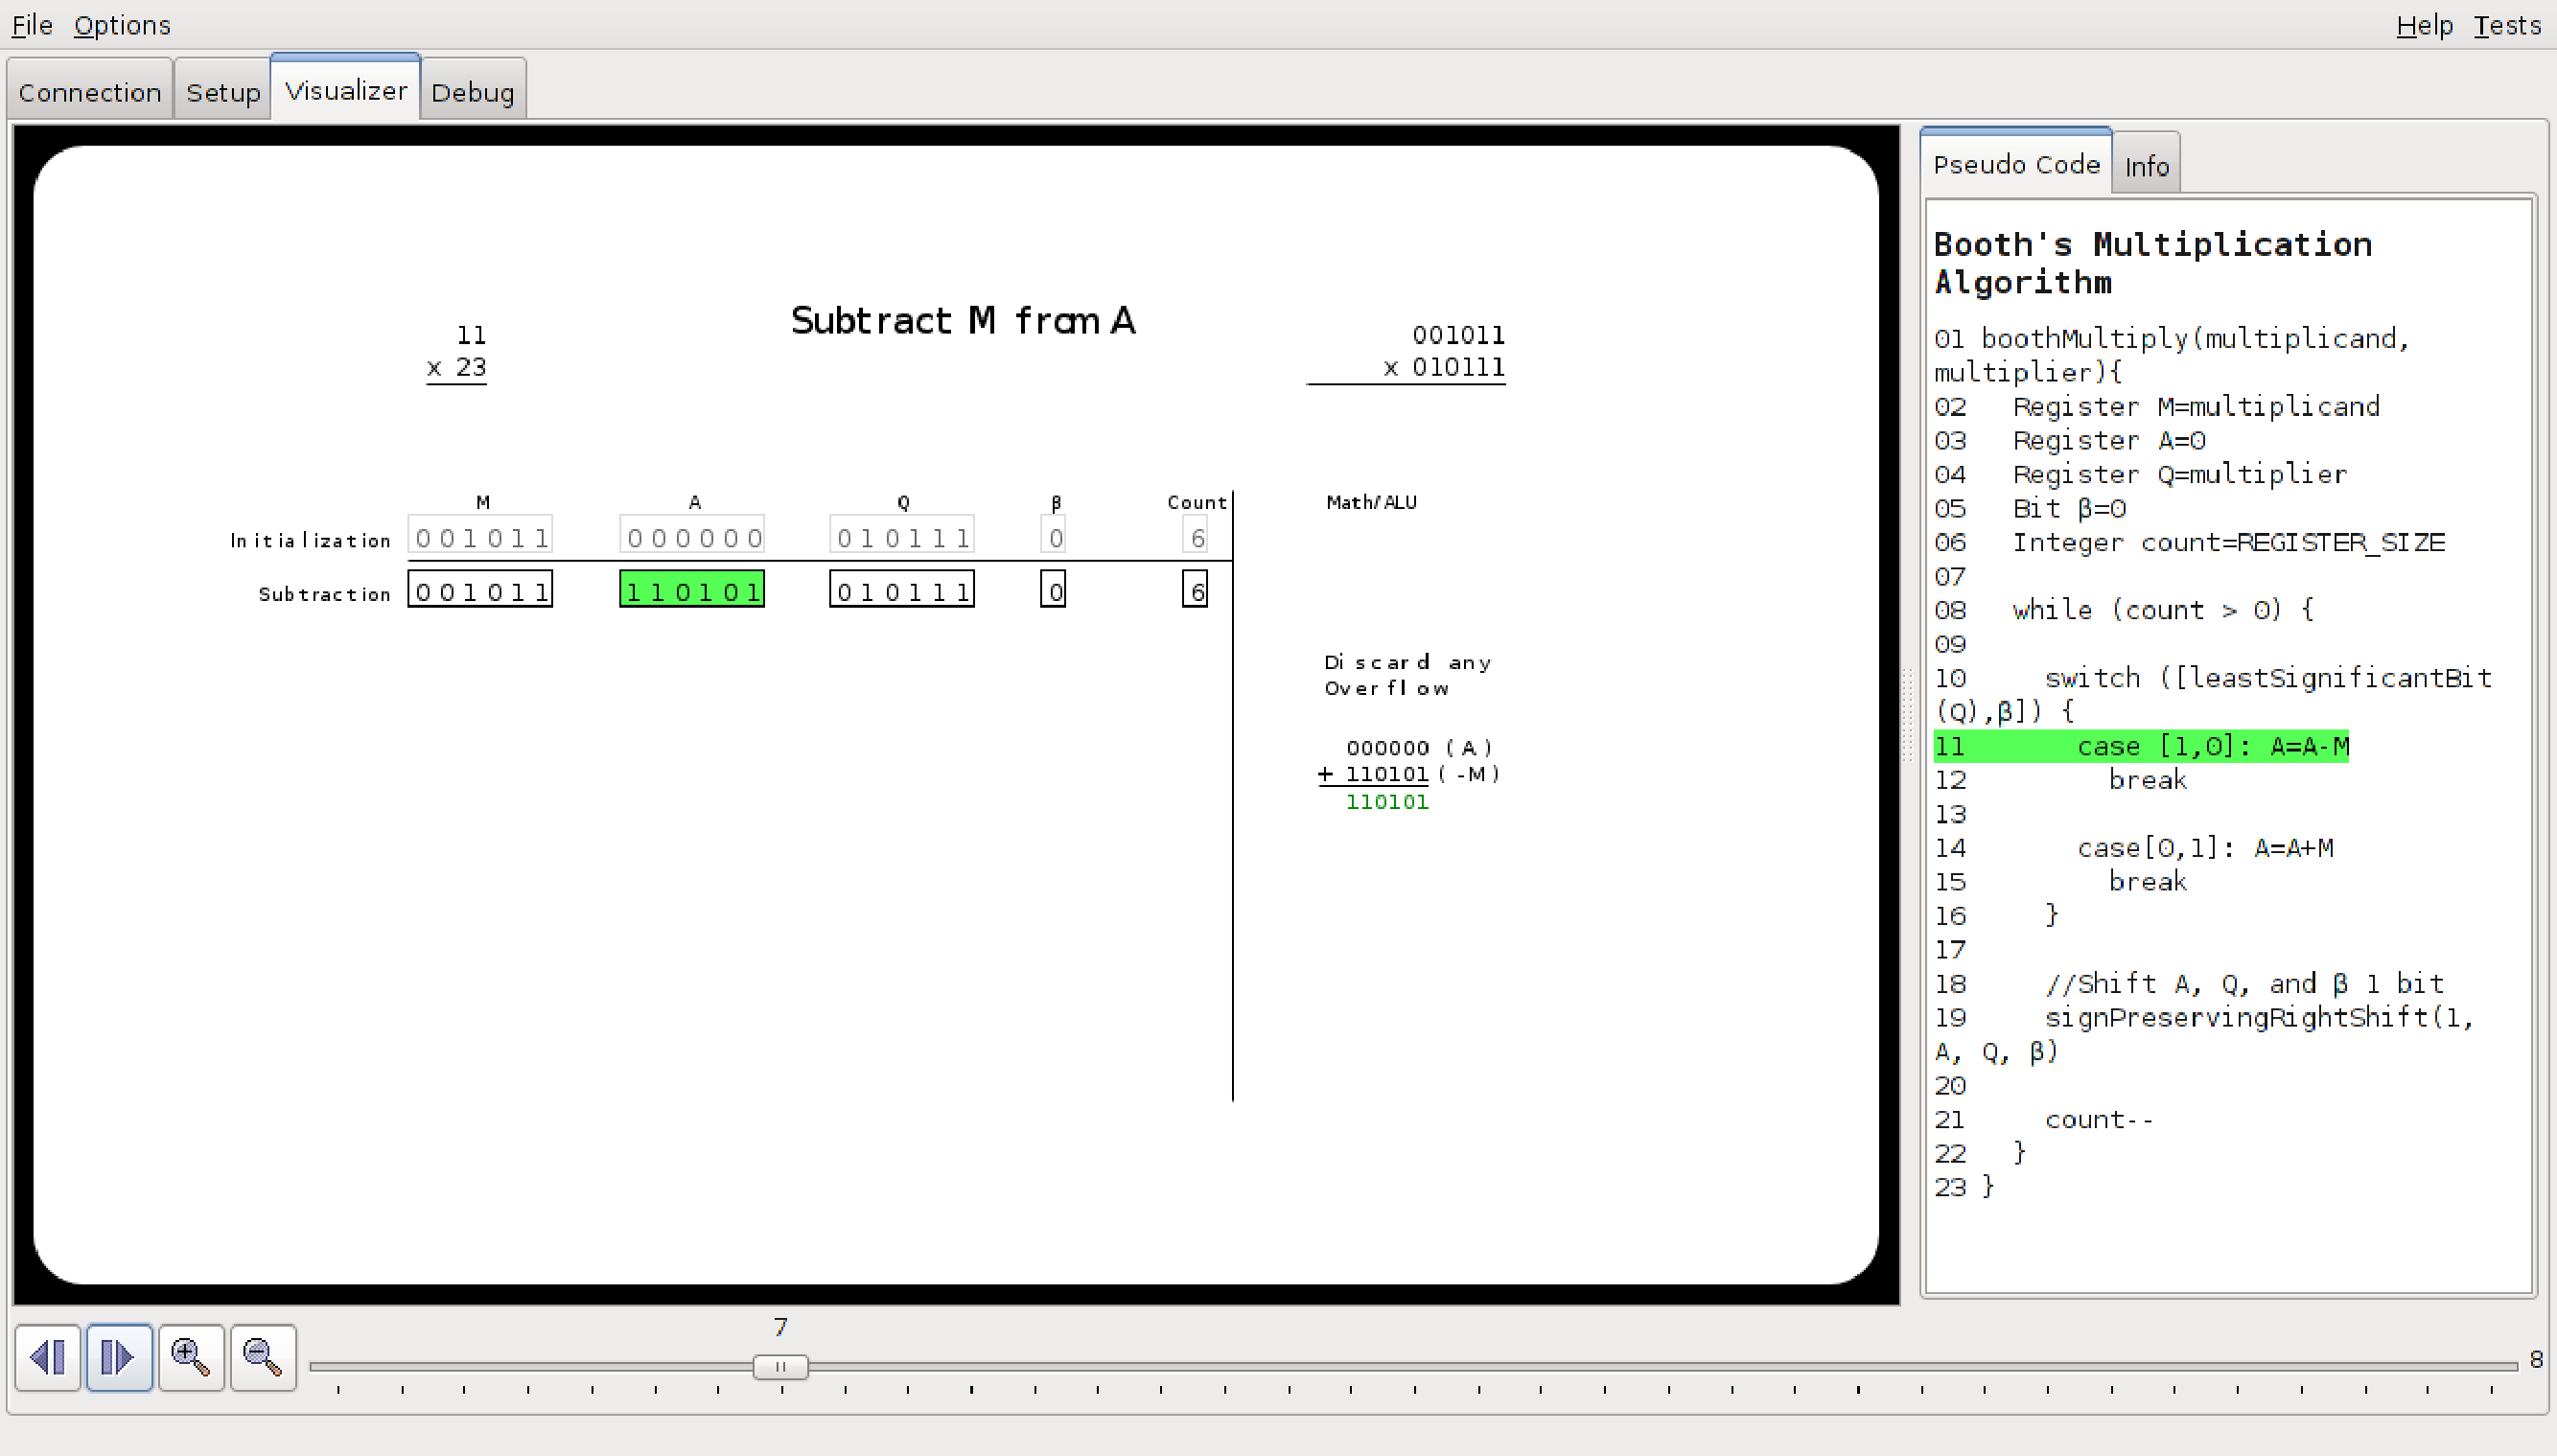
\includegraphics[scale=0.3]{sub.pdf}
\caption{Execute subtraction operation}
\end{figure}

When an arithmetic operation occurs, register A is highlighted green to indicate its updated value.
As always, the last-executed line of pseudo-code is highlighed to match.
The result of the arithmetic in the ``Math/ALU'' column is also highlighted green, except for any overflow, which is discarded.

\pagebreak
\begin{figure}[h]
\centering
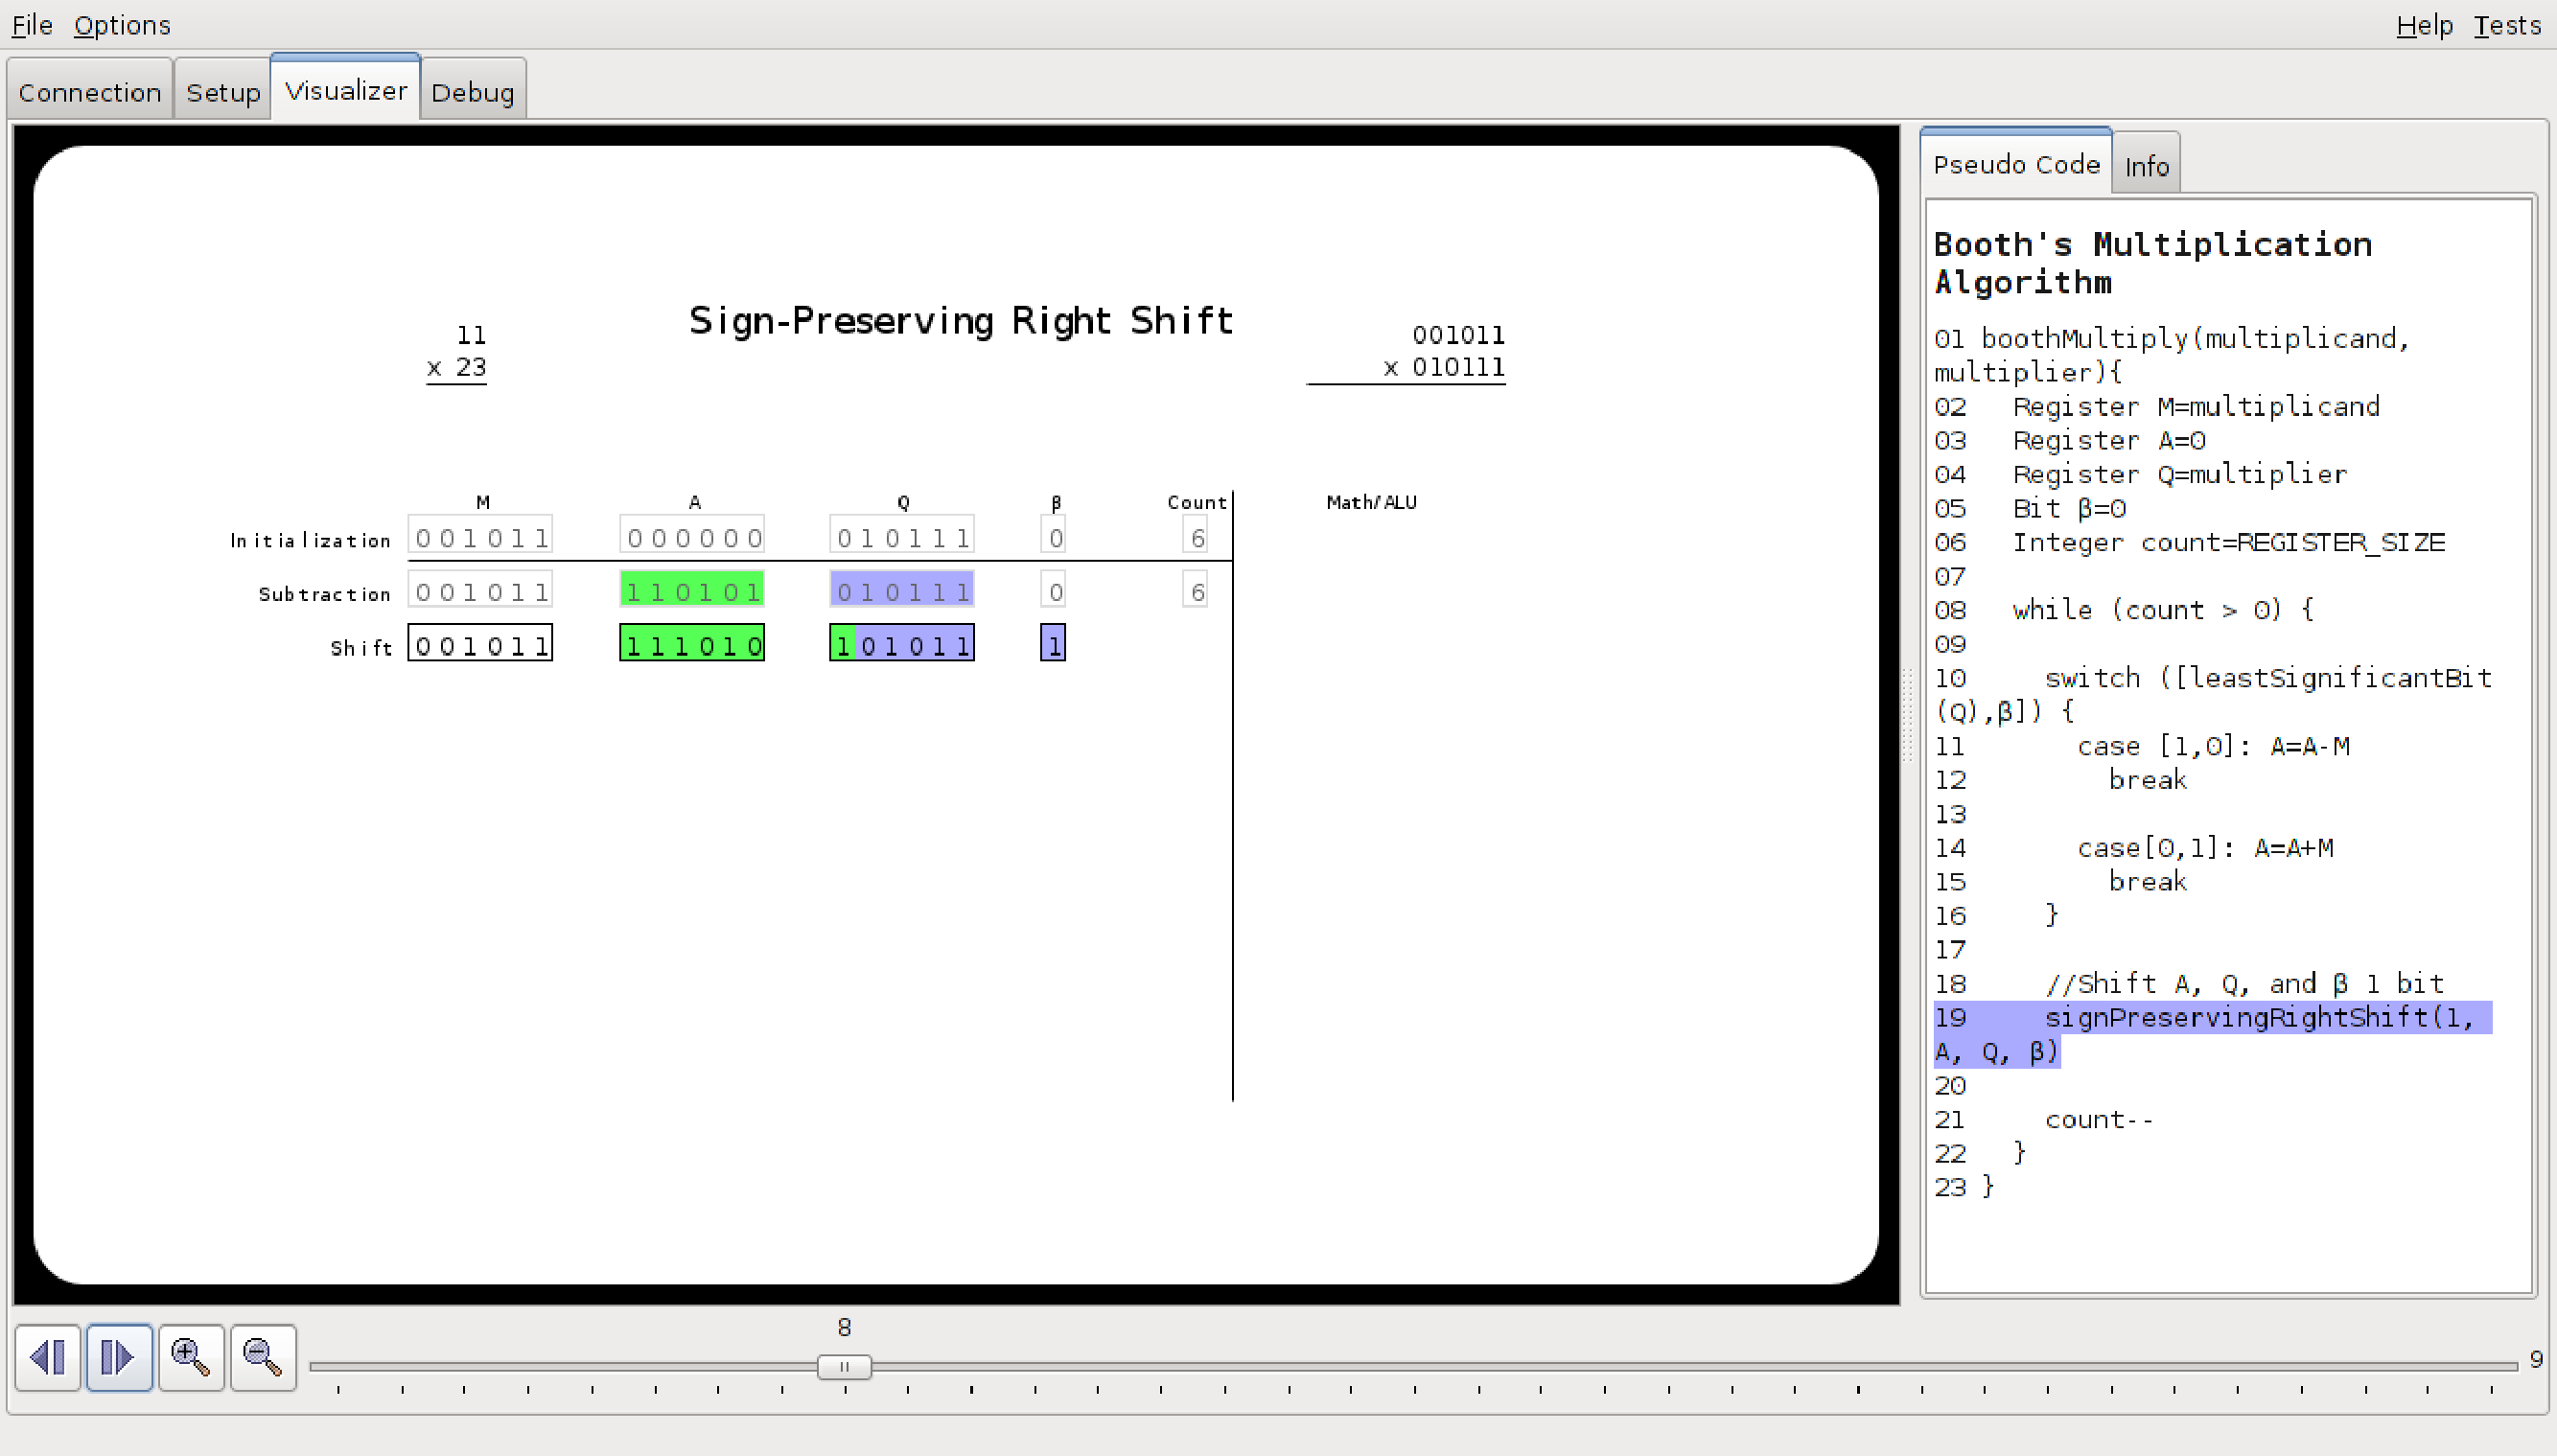
\includegraphics[scale=0.3]{shift.pdf}
\caption{Execute shift operation}
\end{figure}

When a shift operation occurs, the previous values of registers A and Q are highlighted in green and blue, respectively.
The highlighting follows the bits through the shift opperation.
That is, the current values of A and Q are still highlighted in green and blue, with the exception that the the most significant bit of Q is now highlighted green, indicating its value came from register A.
The most-significant bit of A now has the same as the previous most-significant bit of A.
It adopts the green highlighting as the rest of A.%to avoid potential confusion that it may have came from M
\beta is highlighted blue, indicating its value came from register Q.

\pagebreak
Finally, the value of ``Count'' is decremented, and the algorithm returns to the top of the loop.

\begin{figure}[h]
\centering
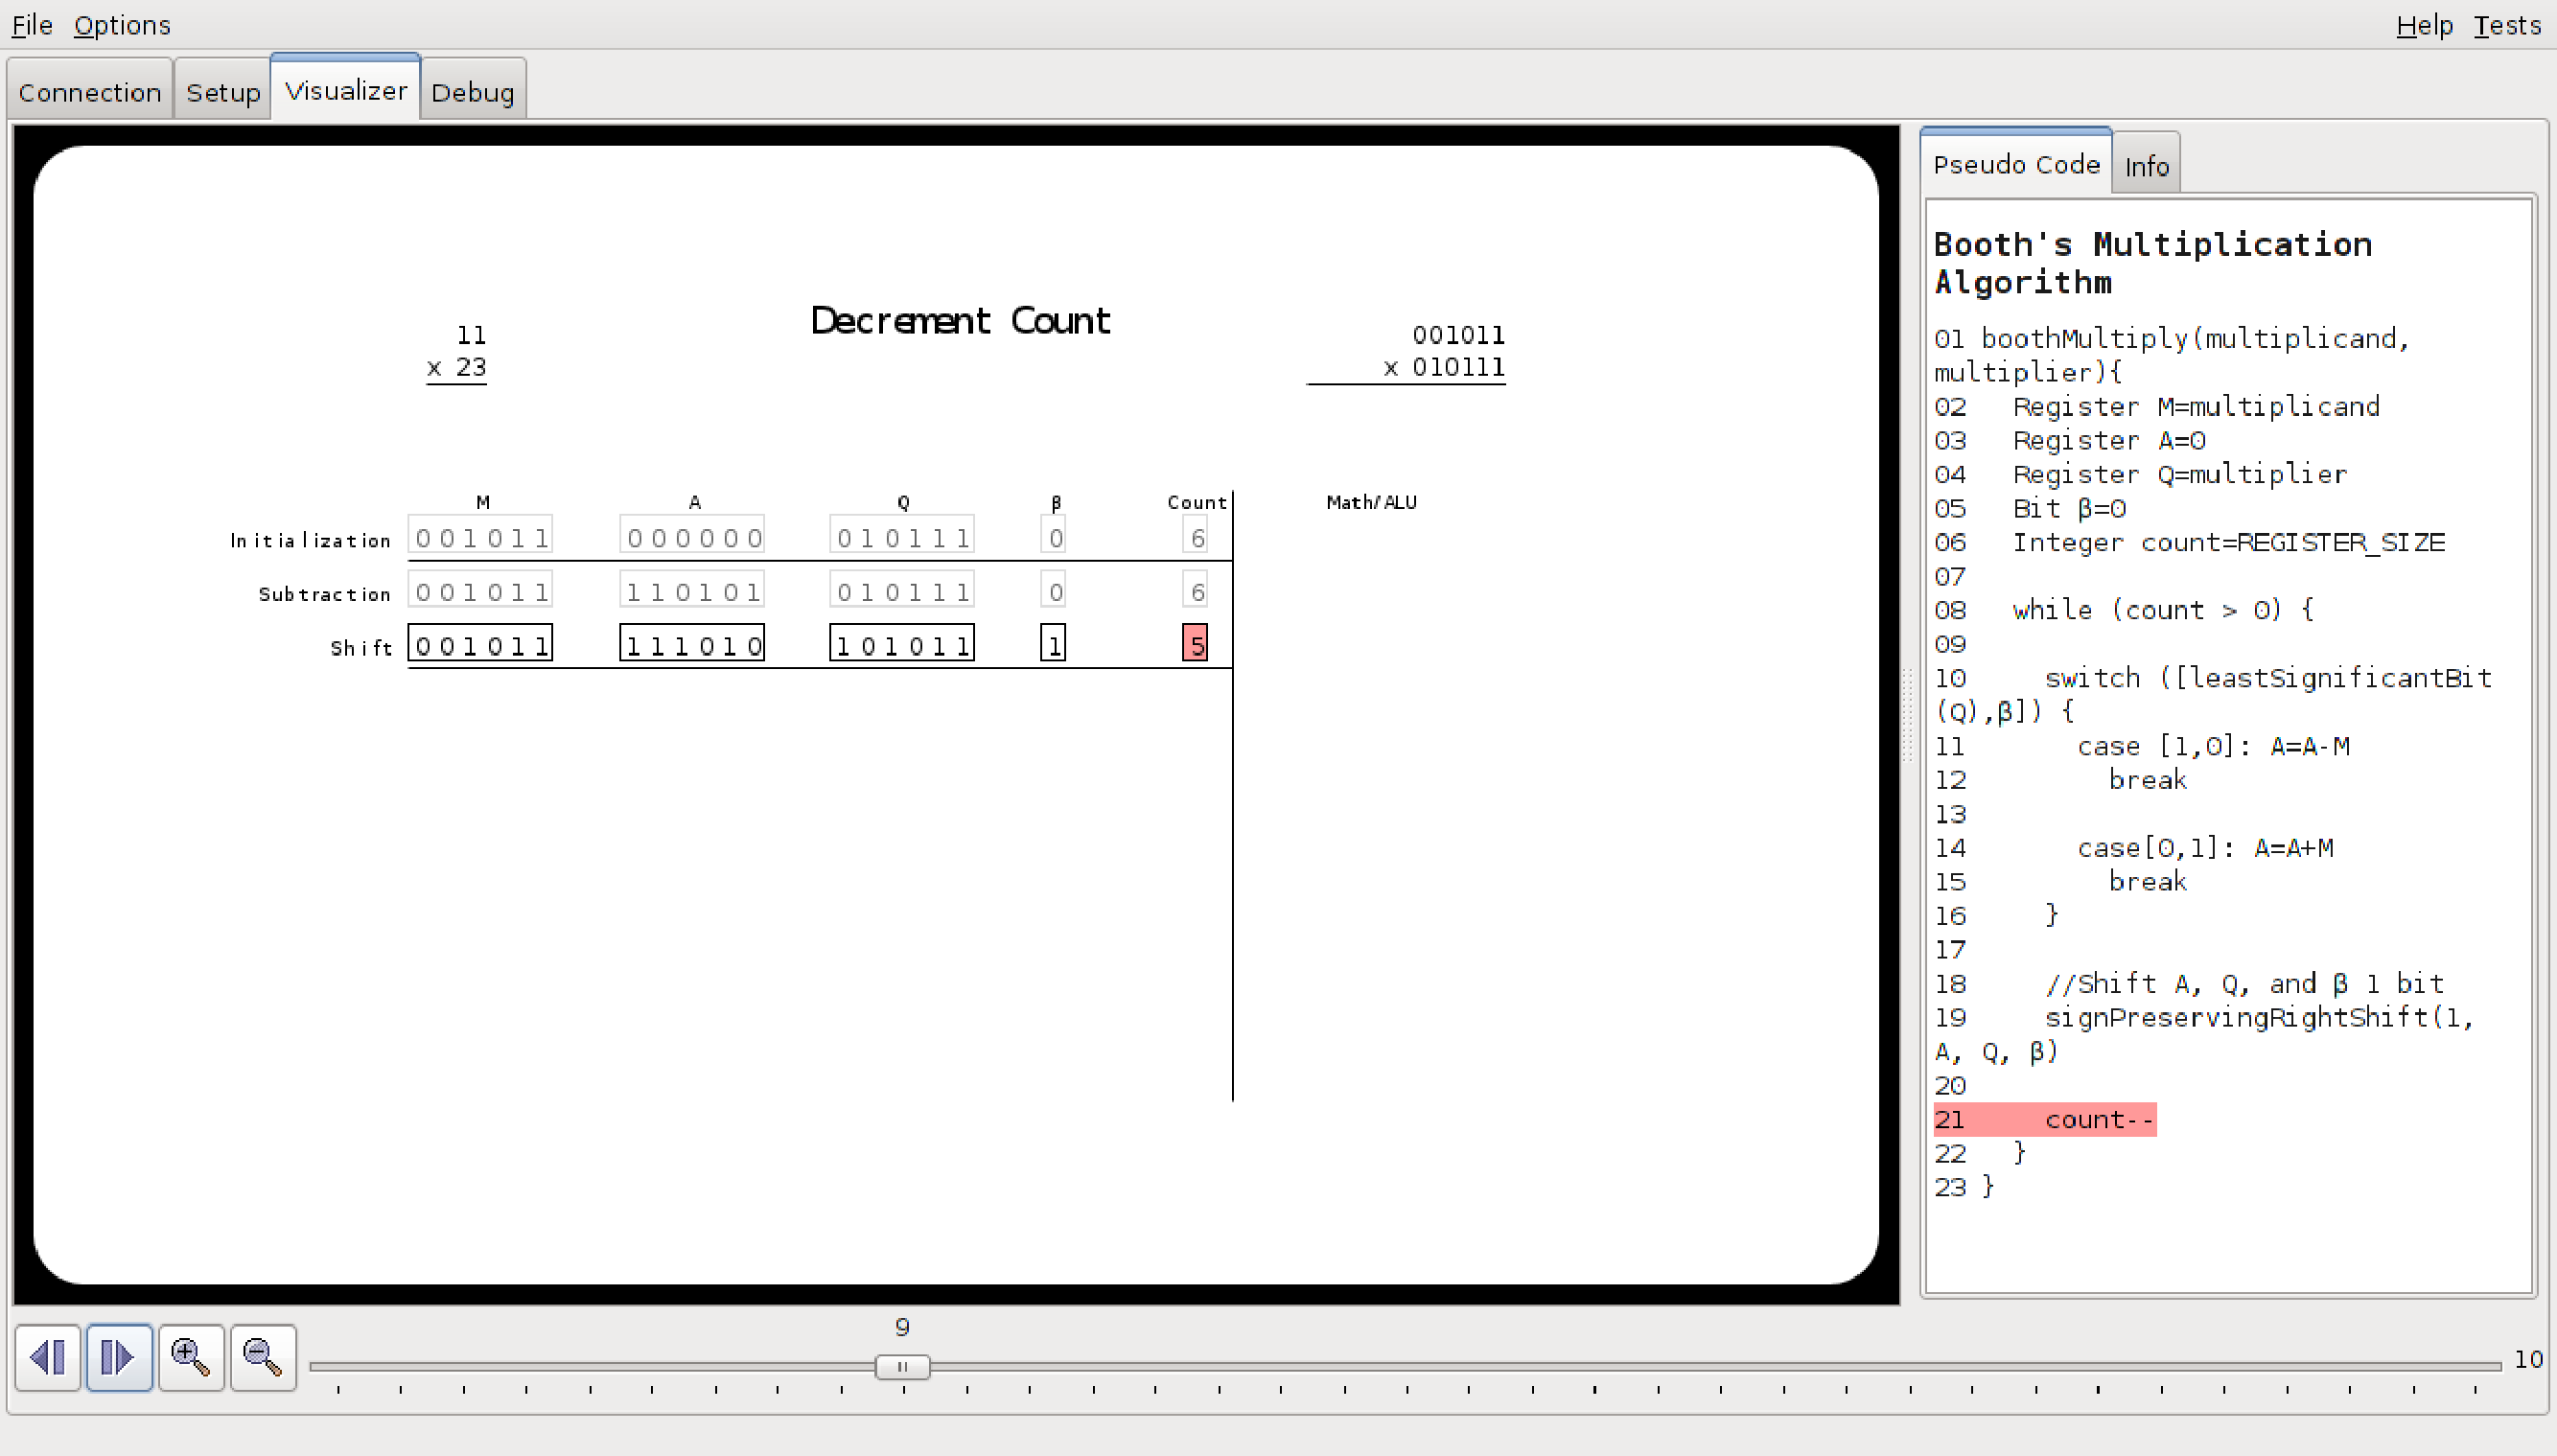
\includegraphics[scale=0.3]{dec.pdf}
\caption{Decrement Count}
\end{figure}

Pop-up questions will appear during the algorithm's visualization.
These questions are randomly selected and are designed to test your understanding of the algorithm.
They come in the following formats: fill in the blank, multiple choice, multiple selection, and true or false.
%The following sentence likely will need to be removed when used with a testing group.
You may disable and enable these questions at any time using the ``Show Questions'' check-box under the ``Options'' menu ; however, since the question are to enhance learning, their use is highly recommended.
%If you prefer, you may disable the questions for the time being by going to the ``Options'' menu and unchecking ``Show Questions''.
%However, once you are more comfortable with the algorithm visualization, it is strongly recommended that you re-enable questions.

\begin{figure}[h]
\centering
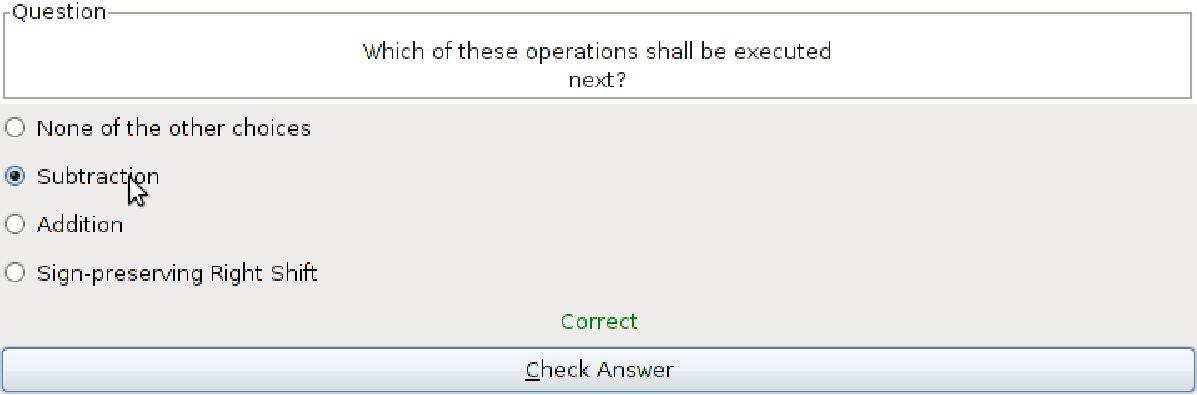
\includegraphics[scale=0.5]{que.pdf}
\caption{An example question}
\end{figure}

\pagebreak

\section{The Visualization's Conclusion}
When ``Count'' is equal to 0, the algorithm exits its loop and completes execution.
The final result of the multiplication spans registers A and Q and is highlighted in green.
The diagrams at the top-left and top-right of the screen are also updated with the decimal and binary result, respectively, which are highlighted in green.

\begin{figure}[h]
\centering
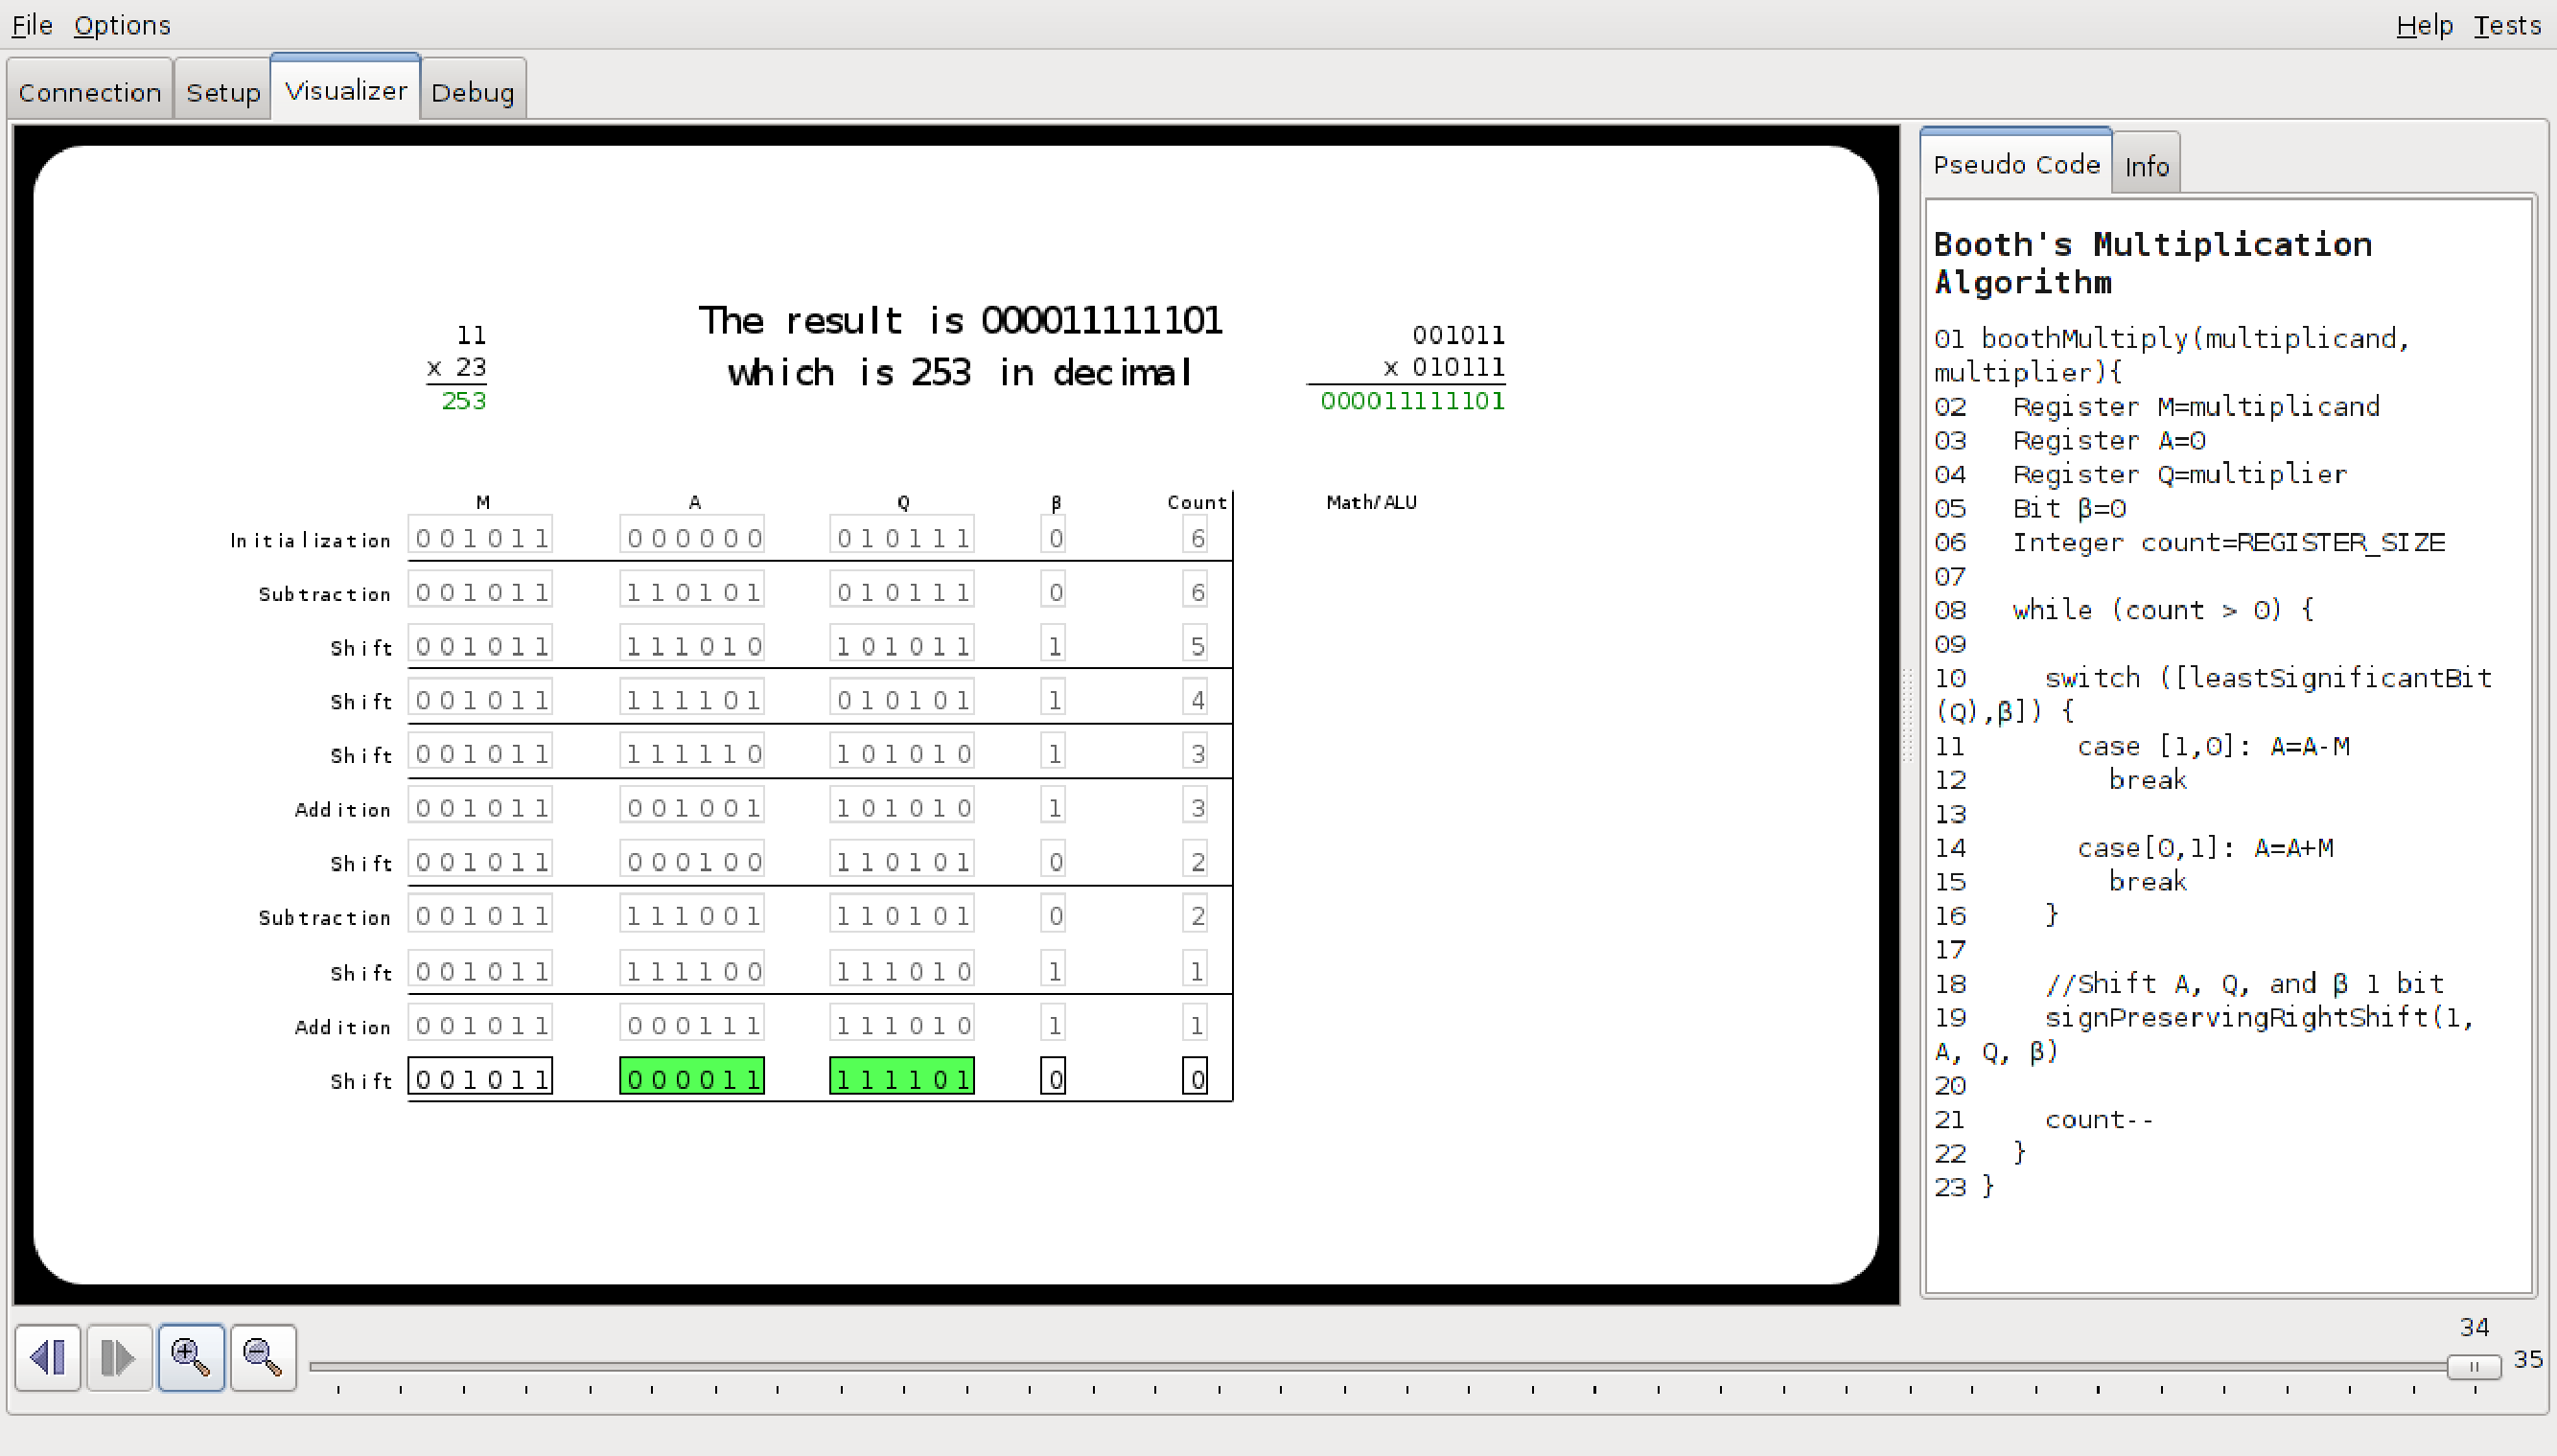
\includegraphics[scale=0.3]{finish.pdf}
\caption{The completed algorithm}
\end{figure}

\end{document}
